\documentclass{article}
%\VignetteIndexEntry{Using KDETrees}
\title{Using KDETrees}
\author{Grady Weyenberg}

\usepackage{Sweave}
\begin{document}
\maketitle

\section{Introduction}
\label{sec:introduction}

KDETrees is a tool for finding discordant phylogenetic trees. It takes as input an {\tt ape::multiPhylo} object, which contains a set of trees, and produces a score for each tree. High scores mean the tree is relatively similar to other trees in the sample, while low scores indicate that the tree in question may be discordant with the others. If desired, a number of low scoring trees may be designated as ``outliers'', which removes their contribution from the calculation. By default the lowest scoring 5\% of the sample is removed.

\section{Basic Use}
\label{sec:use}

\subsection{Importing Trees}
\label{sec:importing-trees}

Trees may be imported using any of the methods provided by {\tt
  ape}. See {\tt ?read.tree} and {\tt ?read.nexus} for examples. To
import the {\tt apicomplexa} dataset, for example, I placed the Newick
tree stringsinto the {\tt apicompexa.tre} file and used the following command:
\begin{Schunk}
\begin{Sinput}
> apicomplexa <- read.tree("apicomplexa.tre")
\end{Sinput}
\end{Schunk}

\subsection{Running kdetrees}
\label{sec:running-kdetrees}

The simplest way to run {\tt kdetrees} is to call the function of the
same name, with the list of trees as the first argument.
\begin{Schunk}
\begin{Sinput}
> result <- kdetrees(apicomplexa)
\end{Sinput}
\end{Schunk}
By default branch lengths are ignored, if you would like to use the
branch length information in the calculation, set the {\tt use.blen}
option to true.
\begin{Schunk}
\begin{Sinput}
> result <- kdetrees(apicomplexa,use.blen=TRUE)
\end{Sinput}
\end{Schunk}
Another important option is the number of ``outlier'' trees which should be
removed from the calculation. This is controlled by the {\tt n} parameter.
\begin{Schunk}
\begin{Sinput}
> result <- kdetrees(apicomplexa,n=12,use.blen=TRUE)
\end{Sinput}
\end{Schunk}
\begin{figure}
  \centering
\begin{Schunk}
\begin{Sinput}
> plot(result)
\end{Sinput}
\end{Schunk}
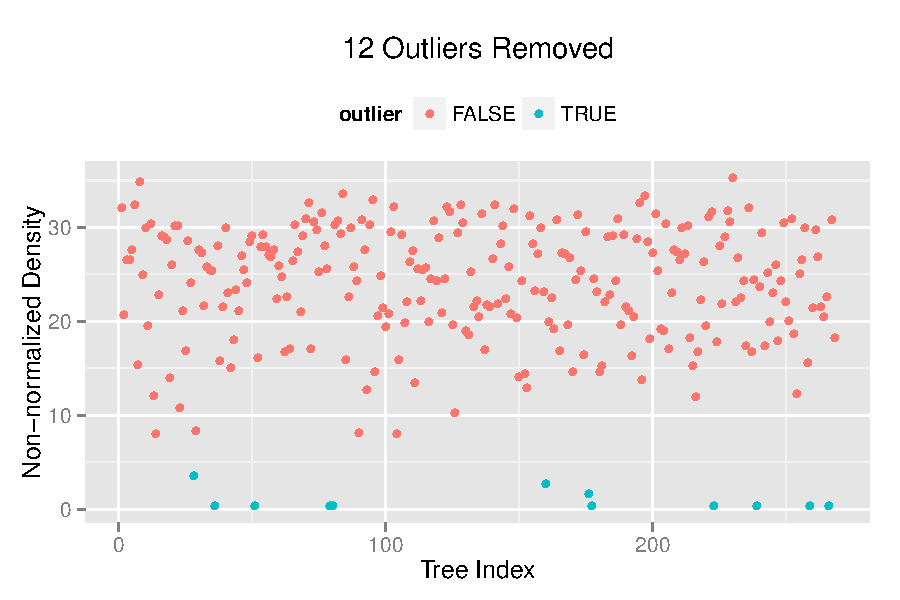
\includegraphics{kdetrees-006}
\begin{Schunk}
\begin{Sinput}
> hist(result)
\end{Sinput}
\end{Schunk}
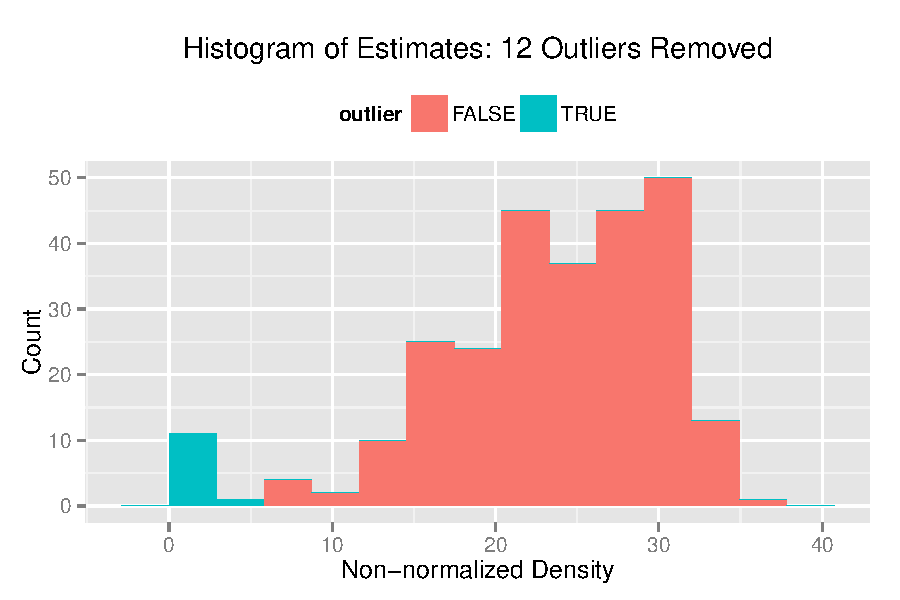
\includegraphics{kdetrees-007}
  \caption{Diagnostic plots can be created with {\tt plot} and {\tt
      hist}. These methods use {\tt ggplot2}, instead of base graphics.}
  \label{fig:diagplots}
\end{figure}

It should be noted that the {\tt plot} and {\tt hist} methods use the
{\tt ggplot2} package, not base graphics. Thus, you can modify them as
you see fit. For example,
\begin{center}
\begin{Schunk}
\begin{Sinput}
> library(ggplot2)
> plot(result) + theme(panel.background=element_blank())
\end{Sinput}
\end{Schunk}
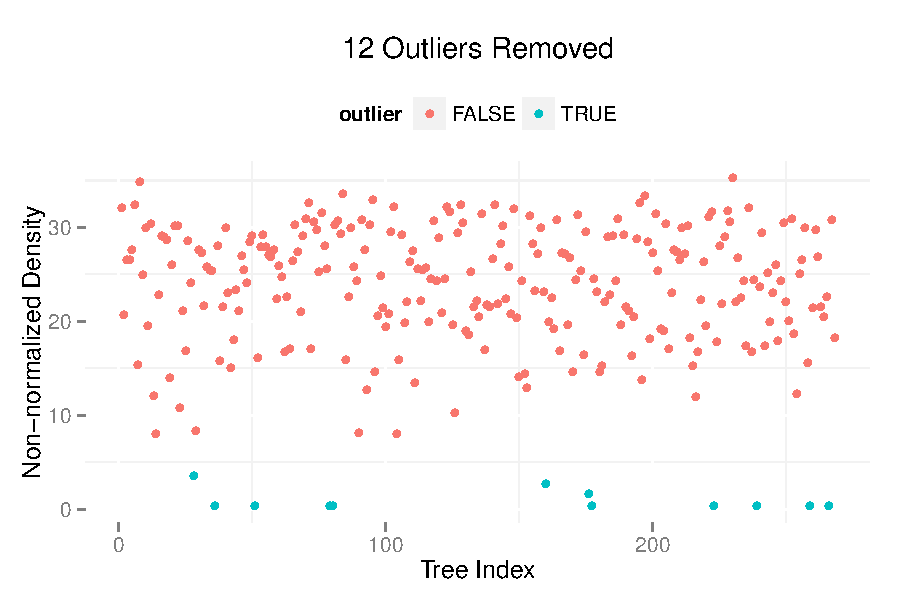
\includegraphics{kdetrees-008}
\end{center}

\subsection{Results}
\label{sec:results}

The result object is a list with three components.
\begin{Schunk}
\begin{Sinput}
> str(result,strict.width="wrap")
\end{Sinput}
\begin{Soutput}
List of 3
$ density : Named num [1:268] 32.1 20.7 26.5 26.5 27.6 ...
..- attr(*, "names")= chr [1:268] "457.tre" "458.tre"
   "459.tre" "460.tre" ...
$ outliers : Named int [1:12] 51 80 266 36 177 79 259 223
   239 176 ...
..- attr(*, "names")= chr [1:12] "515.tre" "547.tre"
   "780.tre" "497.tre" ...
$ bandwidth: Named num [1:268] 1.5 2.85 1.61 1.65 1.63 ...
..- attr(*, "names")= chr [1:268] "457.tre" "458.tre"
   "459.tre" "460.tre" ...
- attr(*, "class")= chr "kdetrees"
\end{Soutput}
\end{Schunk}
The first element, {\tt density}, has the computed score for each tree
in the input list. This is the variable displayed in the diagnostic
plots. The second element {\tt outliers} contains the
indices of the low scoring trees which were not included in the
calculations. We can use this to extract the outlier trees from the
input list.
\begin{Schunk}
\begin{Sinput}
> outlier.trees <- apicomplexa[result$outliers]
\end{Sinput}
\end{Schunk}
One might then wish to look at a plot of the putative outlier
trees. Here I plot the lowest scoring tree in the apicomplexa
dataset. It appears that something bad happened during the
reconstruction of this tree, causing one branch to be much longer
than the others.
\begin{center}
\begin{Schunk}
\begin{Sinput}
> plot(outlier.trees[[1]],"u",no.margin=TRUE)
\end{Sinput}
\end{Schunk}
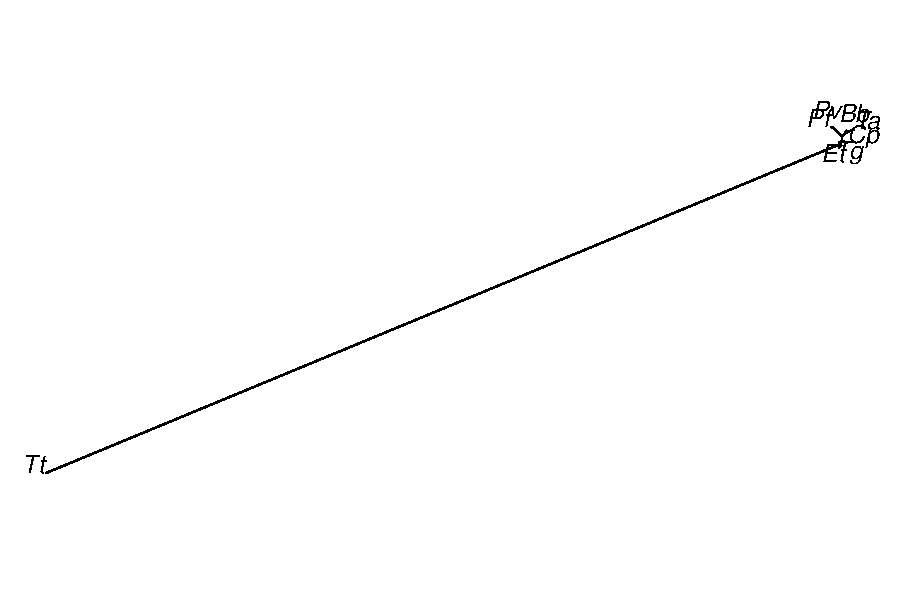
\includegraphics{kdetrees-011}
\end{center}
If you would like to export the outlier trees to a file, you may do
something like the following.
\begin{Schunk}
\begin{Sinput}
> write.tree(outlier.trees,file="outliers.tre")
\end{Sinput}
\end{Schunk}

\section{Shell Script}
\label{sec:shell-script}

The KDETrees package also comes with a bash shell script that calls
{\tt kdetrees} using the Rscript executable. This is a convenience
wrapper for cli users. If you copy this script to a working directory
you can run it as follows.
\begin{Soutput}
$ ./kdetrees -h
Usage: ./kdetrees [options] file [...]
Options:
	-b, --use-branch-lengths
	-n NUM-OUTLIERS, --num-outliers=NUM-OUTLIERS
	-o OUTPUT-PREFIX, --output-prefix=OUTPUT-PREFIX
	-h, --help, Show this help message and exit
\end{Soutput}
This script will read any trees in the file[s] provided as positional
arguments, run kdetrees on them using the options provided, and write
several output files to the current directory. The {\tt outliers.tre}
file will contain newick strings of the outlier trees, these trees are
also rendered in the {\tt outliers.pdf} file. The scatterplot
and histogram pdf filess contain the result of calling {\tt plot} and {\tt
  hist}, respectively, and the {\tt results.csv} file contains the
name, Newick string, and computed score for each tree found.

The final element of the result list {\tt bandwidth} contains the
bandwidths calculated by the nearest-neighbor algorithm. This is
discussed further in the next section.

\section{Advanced Options}
\label{sec:advanced-options}
Currently, kdetrees uses an adaptive bandwidth method based on a
nearest-neighbor calculation by default. It is possible to control the
number of trees used to define the neighborhood, or disable the
adaptive method entirely and provide a constant bandwidth, using the
{\tt bw} parameter. If {\tt bw} is passed as a list, the list is used
as a set of parameters for a call to {\tt bw.nn}. For example, to
change the neighborhood to include 50\% of the sample, instead of the
default 20\%, we would do the following.
\begin{Schunk}
\begin{Sinput}
> kdetrees(apicomplexa,n=12,bw=list(prop=0.5),use.blen=TRUE)
\end{Sinput}
\end{Schunk}
If we wanted to set a constant bandwidth, we simply pass it directly
to {\tt bw}.
\begin{Schunk}
\begin{Sinput}
> kdetrees(apicomplexa,n=12,bw=6,use.blen=TRUE)
\end{Sinput}
\end{Schunk}

The {\tt kdetrees} function is a fairly simple wrapper of a few
component functions.
\begin{Schunk}
\begin{Sinput}
> kdetrees
\end{Sinput}
\begin{Soutput}
function(trees,n=ceiling(0.05*length(trees)),bw=list(),...){
  dm <- dist.diss(trees,...)
  if(is.list(bw)) bw <- do.call(bw.nn,c(list(dm),bw))
  km <- normkern(dm,bw)
  i <- which.min(estimate(km))
  while(length(i) < n){
    j <- which.min(estimate(km[-i,-i]))
    j[1] <- match(names(j),rownames(km))
    i <- c(i,j)
  }
  est <- estimate(km,i)
  out <- list(density=est,outliers=i,bandwidth=bw)
  class(out) <- "kdetrees"
  out
}
<environment: namespace:kdetrees>
\end{Soutput}
\end{Schunk}
Additional control over the method can be achieved by calling the {\tt
  dist.diss}, {\tt normkern}, and {\tt estimate} functions separately,
although this is not recommended unless you know what you are doing.

\end{document}
